\documentclass[12pt]{article}

\usepackage[english]{babel}
\usepackage[utf8]{inputenc}
\usepackage[top=2cm, left=2cm, right=2cm, bottom=2cm]{geometry}
\usepackage[document]{ragged2e}
\usepackage{tikz,minted,times}

\setlength\parindent{0pt}
\sloppy
\usetikzlibrary{automata,positioning,arrows}
\tikzset{node distance=2.5cm,every state/.style={semithick,fill=gray!10},initial text={},double distance=2pt,every edge/.style={draw,->,>=stealth,auto,semithick}}
\usemintedstyle{colorful}

\title{COMP SCI 7411 Event Driven Computing Practice 1 Plan}
\author{Tinson Lai \\ a1812422}
\date{}

\begin{document}

\maketitle

\section{Notations}

The following notations will be used in the diagram.
\begin{itemize}
  \item OPEN and LOCKED are two states defined initially from the question.
  \item Intermediate states will be named $q_i$ where $i$ represents the number of digits in the text box.
  \item $0..9$ means pressing one of the numeric keys once. Similarly, $*$ and $\#$ mean pressing $*$ and $\#$ in the panel respectively.
\end{itemize}

\section{Locking}

\begin{figure}[H]
  \centering
  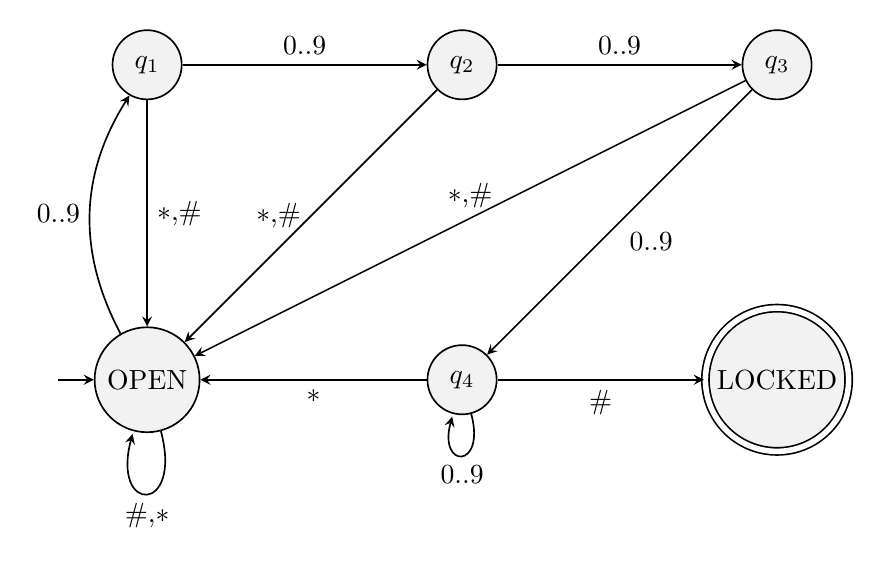
\begin{tikzpicture}
    \node[state, initial] at (0, 0) (open){OPEN};
    \node[state] at (0, 4) (q1){$q_1$};
    \node[state] at (4, 4) (q2){$q_2$};
    \node[state] at (8, 4) (q3){$q_3$};
    \node[state] at (4, 0) (q4){$q_4$};
    \node[state, accepting] at (8, 0) (locked){LOCKED};

    \draw

    (open) edge[bend left, left] node{$0..9$} (q1)
    (q1) edge node{$0..9$} (q2)
    (q2) edge node{$0..9$} (q3)
    (q3) edge node{$0..9$} (q4)
    (q4) edge[loop below] node{$0..9$} (q4)

    (open) edge[loop below] node{$\#$,$*$} (open)
    (q1) edge node{$*$,$\#$} (open)
    (q2) edge[left] node{$*$,$\#$} (open)
    (q3) edge[above] node{$*$,$\#$} (open)
    (q4) edge[below] node{$*$} (open)
    (q4) edge[below] node{$\#$} (locked)

    ;
  \end{tikzpicture}
  \caption{Locking Process}
  \label{fig:locking}
\end{figure}

\section{Unlocking}

\begin{figure}[H]
  \centering
  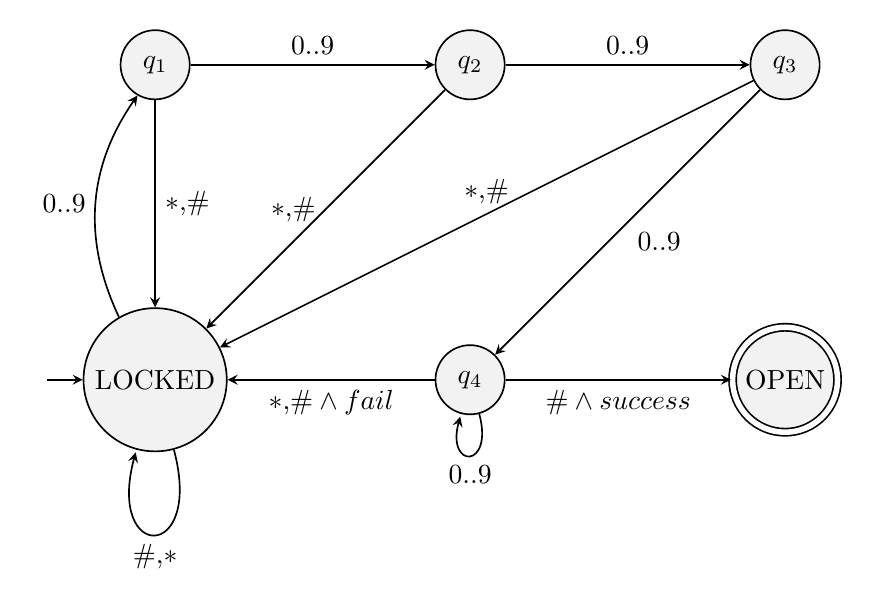
\begin{tikzpicture}
    \node[state, initial] at (0, 0) (locked){LOCKED};
    \node[state] at (0, 4) (q1){$q_1$};
    \node[state] at (4, 4) (q2){$q_2$};
    \node[state] at (8, 4) (q3){$q_3$};
    \node[state] at (4, 0) (q4){$q_4$};
    \node[state, accepting] at (8, 0) (open){OPEN};

    \draw

    (locked) edge[bend left, left] node{$0..9$} (q1)
    (q1) edge node{$0..9$} (q2)
    (q2) edge node{$0..9$} (q3)
    (q3) edge node{$0..9$} (q4)
    (q4) edge[loop below] node{$0..9$} (q4)

    (locked) edge[loop below] node{$\#$,$*$} (locked)
    (q1) edge node{$*$,$\#$} (locked)
    (q2) edge[left] node{$*$,$\#$} (locked)
    (q3) edge[above] node{$*$,$\#$} (locked)
    (q4) edge[below] node{$*$,$\# \wedge fail$} (locked)
    (q4) edge[below] node{$\# \wedge success$} (open)

    ;
  \end{tikzpicture}
  \caption{Unlocking Process}
  \label{fig:unlocking}
\end{figure}

In here, \textbf{\textit{fail}} means the system failed to match the input text with the recorded password, and \textbf{\textit{success}} means the opposite.

\section{Timer}

The timer has a different schedule. It will be triggered by any input of digits if the system is idle. Let's define IDLE state (in Figure \ref{fig:timer}) as a state where no input is currently in the text box and the timer hasn't been started yet. Therefore, either OPEN or LOCKED in both Figure \ref{fig:locking} \& \ref{fig:unlocking} is in timer's IDLE state. Any subsequent input after the first digit by user will not interrupt the timer unless the system status has been effectively reset to idle. A reset can be triggered by pressing either $\#$ or $*$, or if the timer records a duration longer than the set limit.

\begin{figure}[H]
  \centering
  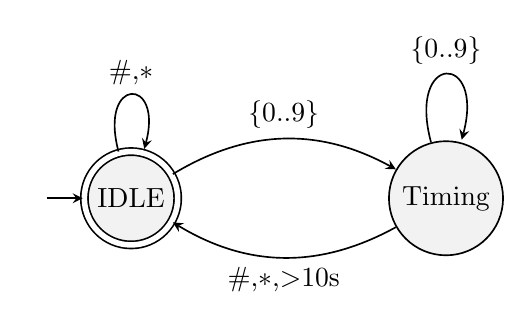
\begin{tikzpicture}
    \node[state, initial, accepting] at (0, 0) (idle){IDLE};
    \node[state] at (4, 0) (timing){Timing};

    \draw

    (idle) edge[loop above] node{$\#$,$*$} (idle)
    (idle) edge[bend left] node{$\left\{0..9\right\}$} (timing)
    (timing) edge[loop above] node{$\left\{0..9\right\}$} (timing)
    (timing) edge[bend left] node{$\#$,$*$,$>$10s} (idle)

    ;
  \end{tikzpicture}
  \caption{Timer}
  \label{fig:timer}
\end{figure}

Here, $>$10s means the timing exceeds 10 seconds, which is a preset limit as required in the question.

\section{Permanent Lock}

Another design choice is that the system will no longer be usable when a set limit (3) of trials is reached. It will ignore all interactive events from users if the system is permanently locked.

\begin{figure}[H]
  \centering
  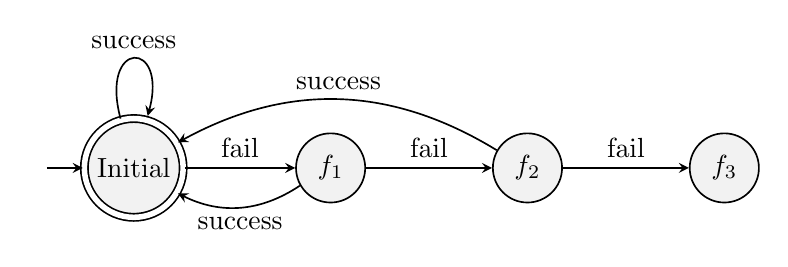
\begin{tikzpicture}
    \node[state, initial, accepting] (initial){Initial};
    \node[state, right of=initial] (f1){$f_1$};
    \node[state, right of=f1] (f2){$f_2$};
    \node[state, right of=f2] (f3){$f_3$};

    \draw

    (initial) edge node{fail} (f1)
    (f1) edge node{fail} (f2)
    (f2) edge node{fail} (f3)

    (initial) edge[loop above] node{success} (initial)
    (f1) edge[bend left, below] node{success} (initial)
    (f2) edge[bend right, above] node{success} (initial)

    ;
  \end{tikzpicture}
  \caption{Permanent Lock}
  \label{fig:permanent}
\end{figure}

\textbf{\textit{success}} and \textbf{\textit{fail}} have the same meanings as in the locking process. A noticeable point is that an invalid length of input will not be counted as a failed trial, which means only three consecutive failed attempts by 4 digits input can lead to the permanent lock. This is an attempt to avoid circumstances such as kids unintentionally trigger the permanent lock because of curiosity. The state $f_3$ in Figure \ref{fig:permanent} is a sink vertex but not an accepting state, which means the system will no longer have any state transitions due to the lock. Refreshing the page will reinitialise everything, which is somewhat similar to real life smart appliances as they will provide certain ways to perform a factory restore. It will discard everything, but the appliance will be usable again.

\section{Implementation Notes}

\begin{itemize}
  \item Pressing $\#$ and $*$ will have the same effect in the state diagram, but in the actual implementation, pressing $\#$ might fire different alerts for different malformed input. Specifically,
  \begin{itemize}
    \item $q_1$, $q_2$ and $q_3$ in both Figure \ref{fig:locking} \& \ref{fig:unlocking} will display an alert for insufficient input length.
    \item $q_4$ in Figure \ref{fig:unlocking} will alert the user for incorrect password. It will also warn the user about the permanent lock if the user have been recorded three failed attempts.
    \item $q_4$ in both Figure \ref{fig:locking} \& \ref{fig:unlocking} will discard any further input by the user, and it will alert the user for unexpected input.
  \end{itemize}
  \item The timer might have a slight offset in timing, but the error is negligible (within 0.1 second which is not perceivable).
  \item The timer will warn the user for taking more than 10 seconds to complete the input, and reset the input as required.
\end{itemize}

\end{document}
